% Options for packages loaded elsewhere
\PassOptionsToPackage{unicode}{hyperref}
\PassOptionsToPackage{hyphens}{url}
%
\documentclass[
]{book}
\usepackage{lmodern}
\usepackage{amssymb,amsmath}
\usepackage{ifxetex,ifluatex}
\ifnum 0\ifxetex 1\fi\ifluatex 1\fi=0 % if pdftex
  \usepackage[T1]{fontenc}
  \usepackage[utf8]{inputenc}
  \usepackage{textcomp} % provide euro and other symbols
\else % if luatex or xetex
  \usepackage{unicode-math}
  \defaultfontfeatures{Scale=MatchLowercase}
  \defaultfontfeatures[\rmfamily]{Ligatures=TeX,Scale=1}
\fi
% Use upquote if available, for straight quotes in verbatim environments
\IfFileExists{upquote.sty}{\usepackage{upquote}}{}
\IfFileExists{microtype.sty}{% use microtype if available
  \usepackage[]{microtype}
  \UseMicrotypeSet[protrusion]{basicmath} % disable protrusion for tt fonts
}{}
\makeatletter
\@ifundefined{KOMAClassName}{% if non-KOMA class
  \IfFileExists{parskip.sty}{%
    \usepackage{parskip}
  }{% else
    \setlength{\parindent}{0pt}
    \setlength{\parskip}{6pt plus 2pt minus 1pt}}
}{% if KOMA class
  \KOMAoptions{parskip=half}}
\makeatother
\usepackage{xcolor}
\IfFileExists{xurl.sty}{\usepackage{xurl}}{} % add URL line breaks if available
\IfFileExists{bookmark.sty}{\usepackage{bookmark}}{\usepackage{hyperref}}
\hypersetup{
  pdftitle={Environmental diversity of microbial eukaryotes},
  pdfauthor={Lab designed by Mahwash Jamy},
  hidelinks,
  pdfcreator={LaTeX via pandoc}}
\urlstyle{same} % disable monospaced font for URLs
\usepackage{color}
\usepackage{fancyvrb}
\newcommand{\VerbBar}{|}
\newcommand{\VERB}{\Verb[commandchars=\\\{\}]}
\DefineVerbatimEnvironment{Highlighting}{Verbatim}{commandchars=\\\{\}}
% Add ',fontsize=\small' for more characters per line
\usepackage{framed}
\definecolor{shadecolor}{RGB}{248,248,248}
\newenvironment{Shaded}{\begin{snugshade}}{\end{snugshade}}
\newcommand{\AlertTok}[1]{\textcolor[rgb]{0.94,0.16,0.16}{#1}}
\newcommand{\AnnotationTok}[1]{\textcolor[rgb]{0.56,0.35,0.01}{\textbf{\textit{#1}}}}
\newcommand{\AttributeTok}[1]{\textcolor[rgb]{0.77,0.63,0.00}{#1}}
\newcommand{\BaseNTok}[1]{\textcolor[rgb]{0.00,0.00,0.81}{#1}}
\newcommand{\BuiltInTok}[1]{#1}
\newcommand{\CharTok}[1]{\textcolor[rgb]{0.31,0.60,0.02}{#1}}
\newcommand{\CommentTok}[1]{\textcolor[rgb]{0.56,0.35,0.01}{\textit{#1}}}
\newcommand{\CommentVarTok}[1]{\textcolor[rgb]{0.56,0.35,0.01}{\textbf{\textit{#1}}}}
\newcommand{\ConstantTok}[1]{\textcolor[rgb]{0.00,0.00,0.00}{#1}}
\newcommand{\ControlFlowTok}[1]{\textcolor[rgb]{0.13,0.29,0.53}{\textbf{#1}}}
\newcommand{\DataTypeTok}[1]{\textcolor[rgb]{0.13,0.29,0.53}{#1}}
\newcommand{\DecValTok}[1]{\textcolor[rgb]{0.00,0.00,0.81}{#1}}
\newcommand{\DocumentationTok}[1]{\textcolor[rgb]{0.56,0.35,0.01}{\textbf{\textit{#1}}}}
\newcommand{\ErrorTok}[1]{\textcolor[rgb]{0.64,0.00,0.00}{\textbf{#1}}}
\newcommand{\ExtensionTok}[1]{#1}
\newcommand{\FloatTok}[1]{\textcolor[rgb]{0.00,0.00,0.81}{#1}}
\newcommand{\FunctionTok}[1]{\textcolor[rgb]{0.00,0.00,0.00}{#1}}
\newcommand{\ImportTok}[1]{#1}
\newcommand{\InformationTok}[1]{\textcolor[rgb]{0.56,0.35,0.01}{\textbf{\textit{#1}}}}
\newcommand{\KeywordTok}[1]{\textcolor[rgb]{0.13,0.29,0.53}{\textbf{#1}}}
\newcommand{\NormalTok}[1]{#1}
\newcommand{\OperatorTok}[1]{\textcolor[rgb]{0.81,0.36,0.00}{\textbf{#1}}}
\newcommand{\OtherTok}[1]{\textcolor[rgb]{0.56,0.35,0.01}{#1}}
\newcommand{\PreprocessorTok}[1]{\textcolor[rgb]{0.56,0.35,0.01}{\textit{#1}}}
\newcommand{\RegionMarkerTok}[1]{#1}
\newcommand{\SpecialCharTok}[1]{\textcolor[rgb]{0.00,0.00,0.00}{#1}}
\newcommand{\SpecialStringTok}[1]{\textcolor[rgb]{0.31,0.60,0.02}{#1}}
\newcommand{\StringTok}[1]{\textcolor[rgb]{0.31,0.60,0.02}{#1}}
\newcommand{\VariableTok}[1]{\textcolor[rgb]{0.00,0.00,0.00}{#1}}
\newcommand{\VerbatimStringTok}[1]{\textcolor[rgb]{0.31,0.60,0.02}{#1}}
\newcommand{\WarningTok}[1]{\textcolor[rgb]{0.56,0.35,0.01}{\textbf{\textit{#1}}}}
\usepackage{longtable,booktabs}
% Correct order of tables after \paragraph or \subparagraph
\usepackage{etoolbox}
\makeatletter
\patchcmd\longtable{\par}{\if@noskipsec\mbox{}\fi\par}{}{}
\makeatother
% Allow footnotes in longtable head/foot
\IfFileExists{footnotehyper.sty}{\usepackage{footnotehyper}}{\usepackage{footnote}}
\makesavenoteenv{longtable}
\usepackage{graphicx,grffile}
\makeatletter
\def\maxwidth{\ifdim\Gin@nat@width>\linewidth\linewidth\else\Gin@nat@width\fi}
\def\maxheight{\ifdim\Gin@nat@height>\textheight\textheight\else\Gin@nat@height\fi}
\makeatother
% Scale images if necessary, so that they will not overflow the page
% margins by default, and it is still possible to overwrite the defaults
% using explicit options in \includegraphics[width, height, ...]{}
\setkeys{Gin}{width=\maxwidth,height=\maxheight,keepaspectratio}
% Set default figure placement to htbp
\makeatletter
\def\fps@figure{htbp}
\makeatother
\setlength{\emergencystretch}{3em} % prevent overfull lines
\providecommand{\tightlist}{%
  \setlength{\itemsep}{0pt}\setlength{\parskip}{0pt}}
\setcounter{secnumdepth}{5}
\usepackage{booktabs}
\usepackage[]{natbib}
\bibliographystyle{plainnat}

\title{Environmental diversity of microbial eukaryotes}
\author{Lab designed by Mahwash Jamy}
\date{2021-11-17}

\usepackage{amsthm}
\newtheorem{theorem}{Theorem}[chapter]
\newtheorem{lemma}{Lemma}[chapter]
\newtheorem{corollary}{Corollary}[chapter]
\newtheorem{proposition}{Proposition}[chapter]
\newtheorem{conjecture}{Conjecture}[chapter]
\theoremstyle{definition}
\newtheorem{definition}{Definition}[chapter]
\theoremstyle{definition}
\newtheorem{example}{Example}[chapter]
\theoremstyle{definition}
\newtheorem{exercise}{Exercise}[chapter]
\theoremstyle{definition}
\newtheorem{hypothesis}{Hypothesis}[chapter]
\theoremstyle{remark}
\newtheorem*{remark}{Remark}
\newtheorem*{solution}{Solution}
\begin{document}
\maketitle

{
\setcounter{tocdepth}{1}
\tableofcontents
}
\hypertarget{before-you-start-the-lab}{%
\chapter{Before you start the lab}\label{before-you-start-the-lab}}

This lab will introduce you to metabarcoding. Investigating this ``hidden diversity'' often relies heavily on bioinformatics. Here, most of the analyses have already been carried out for you, and the focus is on interpreting the results of the analyses. All graphs in this practical have been generated in R. The code is visible for those interested (don't worry if it does not make sense! The goal here is to interpret results) - but you can hide the code by clicking the \texttt{Hide} button above each code chunk.

To complete this lab, answer all questions (in bold) and discuss them with your teaching assistant at the end of the lab.

Good luck! :)

\hypertarget{learning-outcomes}{%
\section{Learning outcomes}\label{learning-outcomes}}

After completing this lab, you will be able to:

\begin{itemize}
\tightlist
\item
  Explain how DNA can be used to study microbial diversity in a high-throughput way and contrast it with using morphology\\
\item
  Use given sequences to BLAST against a reference database and identify the corresponding organism\\
\item
  Explain the concept of metabarcoding, and assess its power and limitations\\
\item
  Classify sequences based on phylogenetic placement\\
\item
  Analyse the ecology of taxa of interest using sequence information\\
\item
  Analyse and assess how different microbial communities are structured
\end{itemize}

\hypertarget{motivation}{%
\section{Motivation}\label{motivation}}

Microbes run the world! Protists and fungi play crucial ecological roles such as primary production, consumers and decomposers. But how do we study them given that they are so small? Furthermore, most of them are difficult to culture. One method is: using a metabarcoding approach!

\begin{figure}
\centering
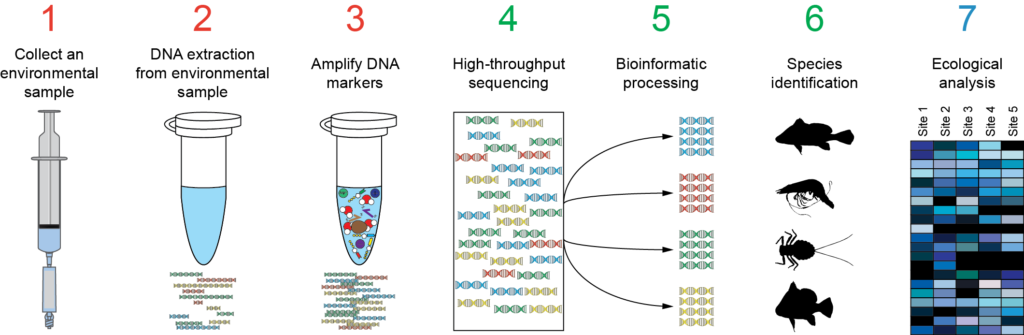
\includegraphics{images/metabarcoding_workflow.png}
\caption{Fig. 1: Metabarcoding overview (source:\url{http://www.naturemetrics.co.uk})}
\end{figure}

Figure 1 shows an overview of the metabarcoding approach. The most commonly used DNA barcode for microbial eukaryotes is the \textbf{18S rDNA} gene (though it should be noted that the internal transcribed spacer, ITS, is more commonly used for fungi). In this lab, we will focus on the 18S gene using subsets of published sequencing data from: global marinesampling expeditions such as \href{https://www.science.org/doi/10.1126/science.1261605}{Tara Oceans} and the \href{https://www.nature.com/articles/s41396-019-0506-9}{Malaspina Expedition}, \href{https://www.mdpi.com/2076-2607/8/4/543}{freshwater from Lake Baikal}, and \href{https://www.nature.com/articles/s41559-017-0091}{soils from Neotropical forests}.

\hypertarget{the-data}{%
\chapter{The data}\label{the-data}}

In this section, you will work with a subset of data from the Tara Oceans Expedition (de Vargas et al.~2015, \emph{Science}). For this lab, we have gathered sequences from two marine environments: Coral Reefs, and Open Ocean. Each environment is represented by three stations each, meaning that you will be working with data from 6 stations in total. The location of these stations is shown in the map in Figure 2.

\begin{figure}
\centering
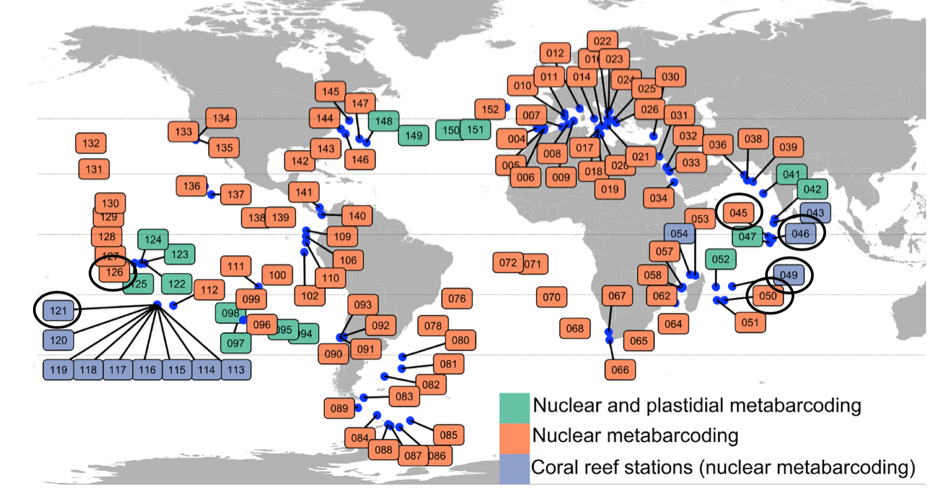
\includegraphics{images/chosen_stations.png}
\caption{Fig. 2: Tara Ocean sampling stations (adapted with permission from Decelle et al.~2018, \emph{Cell}). Here, we will focus on the circled stations.}
\end{figure}

The Tara Oceans project used a region (V9) of the 18S gene (the Small Ribosomal Subunit gene in eukaryotes, see Figure 3 below) as a metabarcode.

\includegraphics{images/18S.png}

These sequences were correspond to organisms living in surface water (\textasciitilde{} 7 m depth) collected from the six stations. The water was size fractionated to recover biodiversity from major organismal size fractions: pico-nanoplankton (0.8 to 5 microns), nanoplankton (5 to 20 microns), microplankton (20 to 180 microns) and mesoplankton (180 to 2000 microns). \emph{However, in this lab we have merged all the size fractions for simplicity.}

\hypertarget{getting-a-feel-for-your-data}{%
\section{Getting a feel for your data}\label{getting-a-feel-for-your-data}}

Normally, we start our data analysis with a LOT of reads or metabarcodes. The first step is to filter these reads based on quality and then cluster them into biologically meaningful Operational Taxonomic Units (OTUs). Here, in the interest of time, we have already cleaned the reads and clustered them into OTUs.

\begin{Shaded}
\begin{Highlighting}[]
\CommentTok{# read table containing metadata about stations}
\NormalTok{otus <-}\StringTok{ }\KeywordTok{read.csv}\NormalTok{(}\StringTok{"data/metadata.txt"}\NormalTok{, }\DataTypeTok{header=}\NormalTok{T, }\DataTypeTok{sep =} \StringTok{"}\CharTok{\textbackslash{}t}\StringTok{"}\NormalTok{)}
\NormalTok{otus}
\end{Highlighting}
\end{Shaded}

\begin{verbatim}
##      station no_of_OTUs no_of_reads       type        time.date Temp..Celcius.
## 1  station45      16376     9777277 open_ocean 2010-04-13T03:21       30.59345
## 2  station50      10532     2742747 open_ocean 2010-05-09T05:30       27.54930
## 3 station126      31777     4930749 open_ocean 2011-08-28T18:05       26.68965
## 4 station121      11639     2396972      coral 2011-07-09T17:47       24.23274
## 5  station46      15309    15360520      coral 2010-04-15T02:01       30.12475
## 6  station49      12782     1722440      coral 2010-04-23T10:10       28.27290
\end{verbatim}

\textbf{Questions:}\\
\textbf{1. The Tara Oceans Project found \textasciitilde110,000 OTUs in total from surface waters of tropical and temperate oceans. Pick any \emph{one} of the six stations. What proportion of total species diversity is present at that station?}

\hypertarget{what-do-these-otus-represent-anyway}{%
\section{What do these OTUs represent anyway?}\label{what-do-these-otus-represent-anyway}}

OTUs are often defined using sequence similarity thresholds (traditionally sequences more than 97\% dissimilar are treated as belonging to different species, though other criteria are also frequently used). But what do these OTUs actually represent? Does OTU = species? Here we will evaluate what OTUs represent using several different examples of described species.

\hypertarget{scenario-1}{%
\subsection{Scenario 1}\label{scenario-1}}

You isolate two cells from soil samples in Nova Scotia, Canada and photograph them using contrast light microscopy (Figure 4).

\begin{figure}
\centering
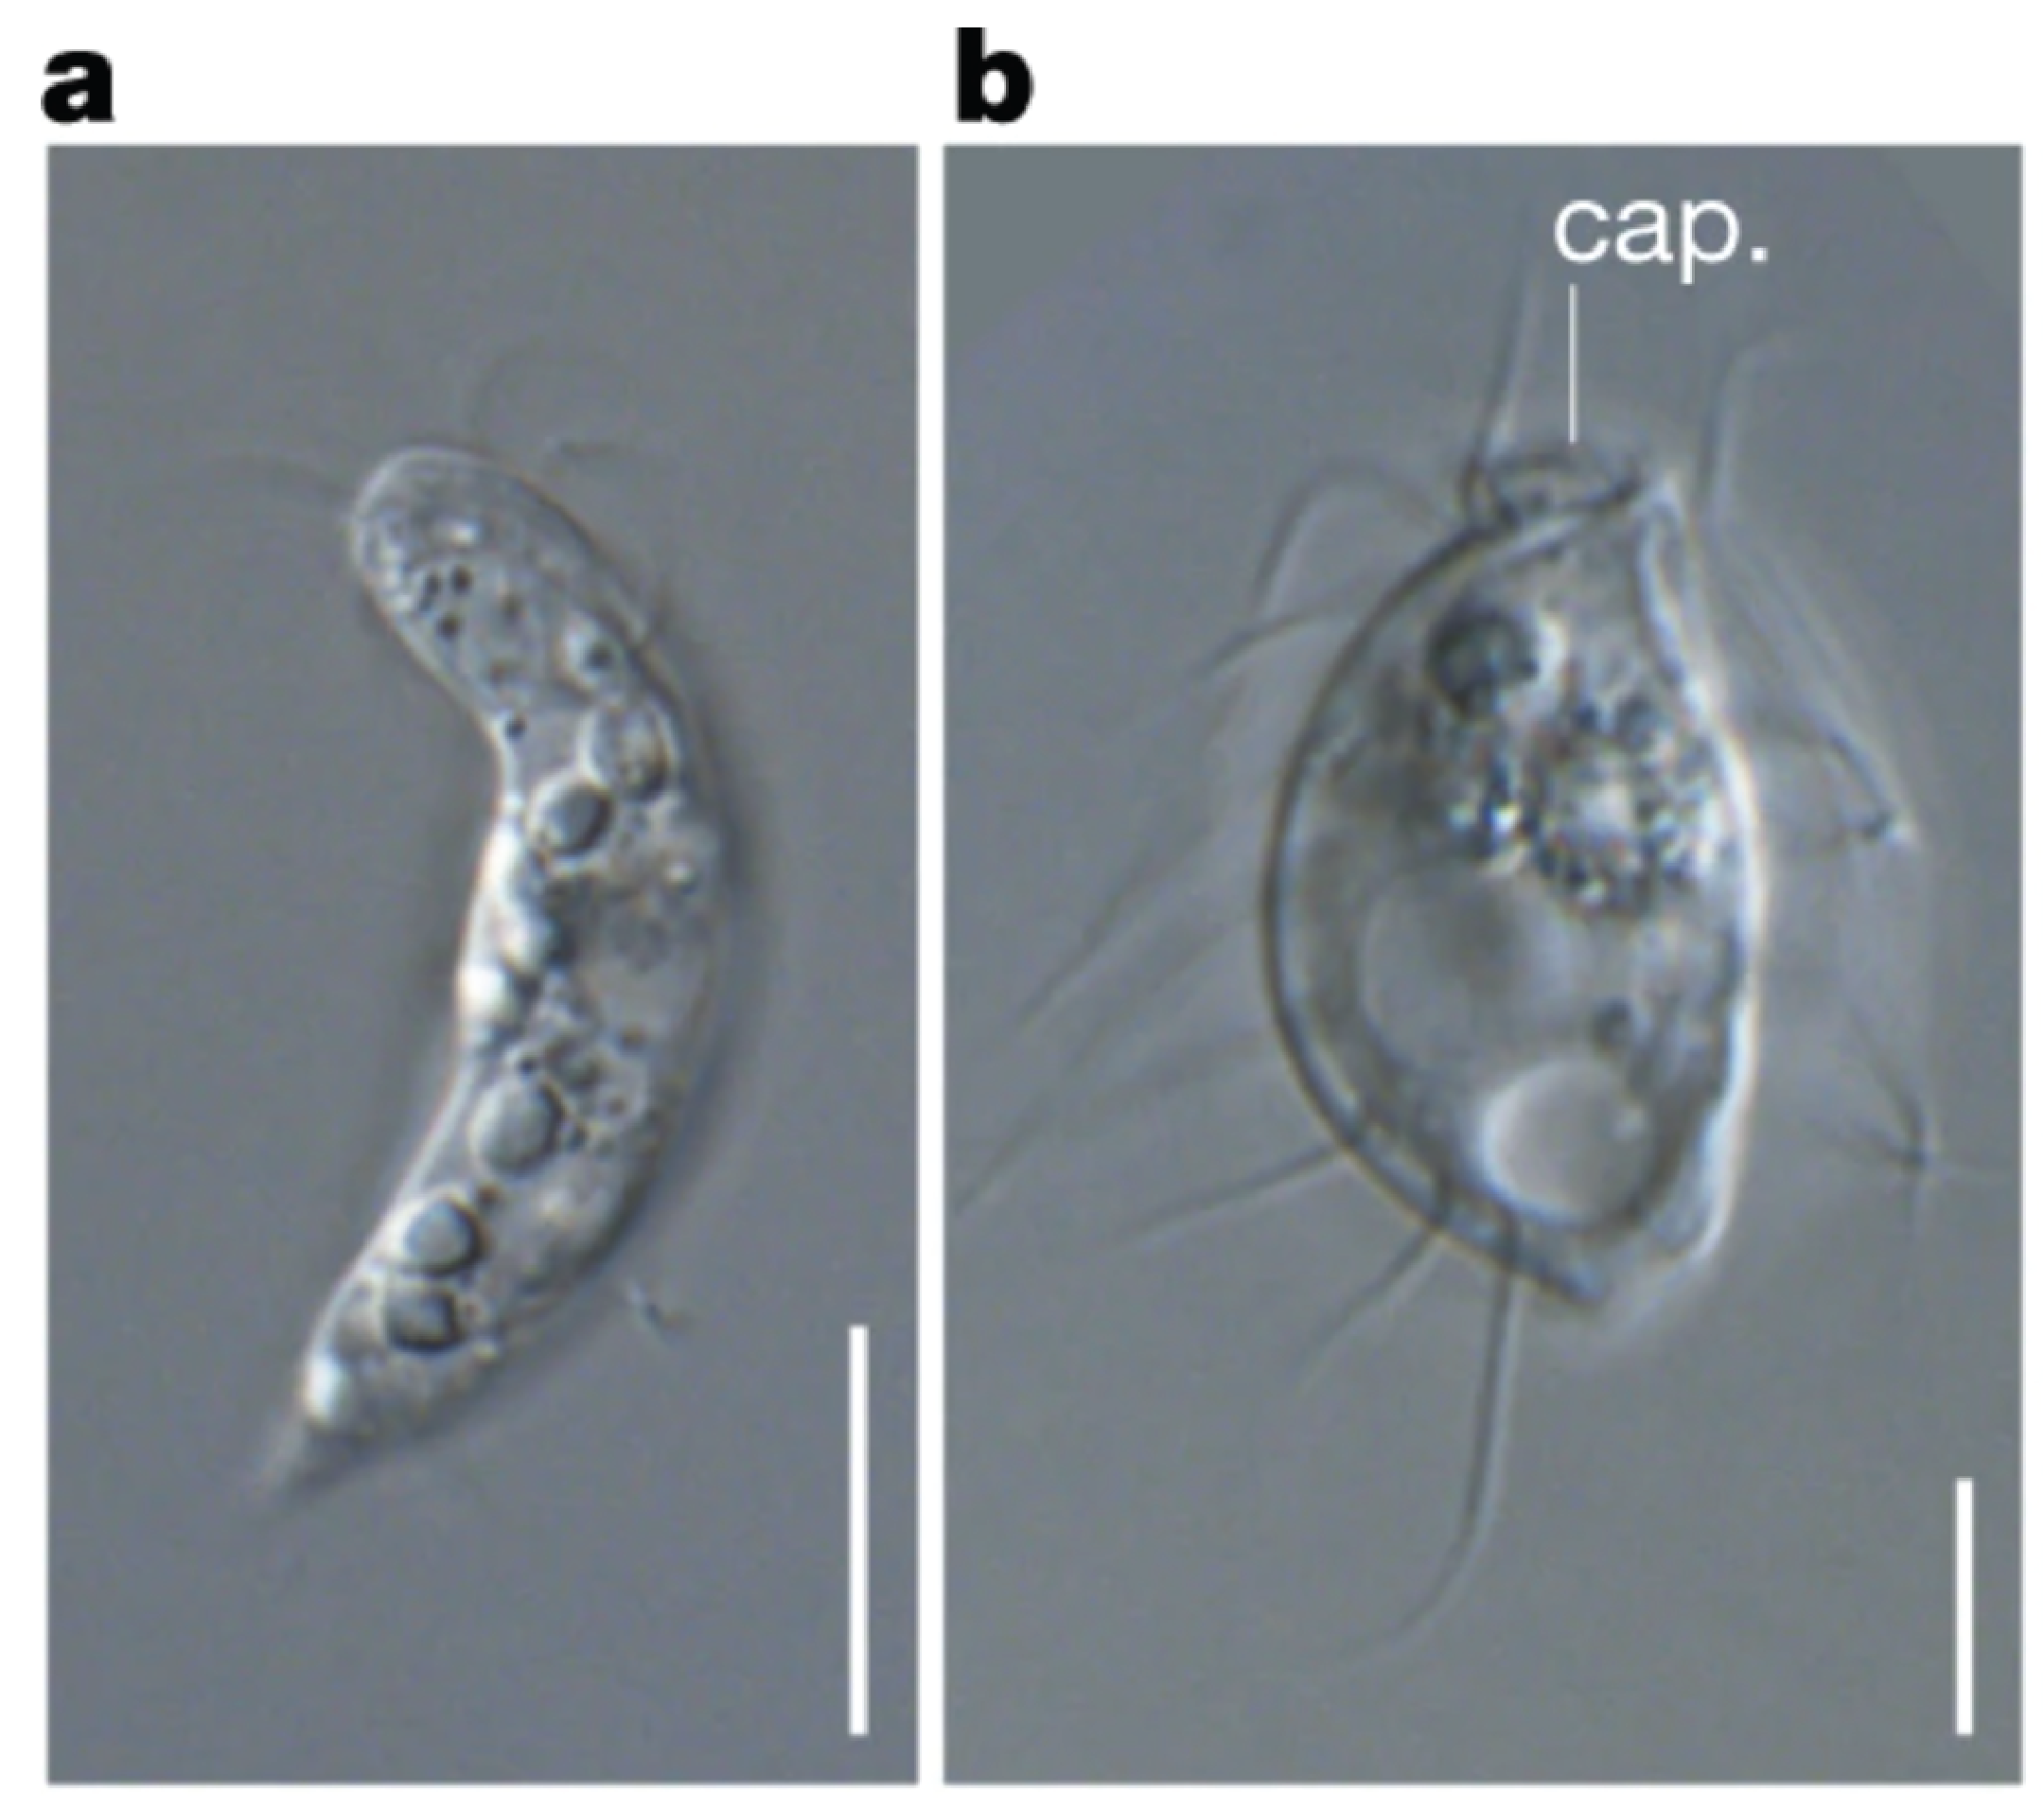
\includegraphics{images/hemimastigotes.png}
\caption{Fig. 4: Two protist cells from soil, Canada (from Lax et al.~2018, \emph{Nature}). Size of scale bar in \textbf{a} is 10 μm, and 5 μm in \textbf{b}.}
\end{figure}

\hypertarget{cross}{%
\chapter{Cross-references}\label{cross}}

Cross-references make it easier for your readers to find and link to elements in your book.

\hypertarget{chapters-and-sub-chapters}{%
\section{Chapters and sub-chapters}\label{chapters-and-sub-chapters}}

There are two steps to cross-reference any heading:

\begin{enumerate}
\def\labelenumi{\arabic{enumi}.}
\tightlist
\item
  Label the heading: \texttt{\#\ Hello\ world\ \{\#nice-label\}}.

  \begin{itemize}
  \tightlist
  \item
    Leave the label off if you like the automated heading generated based on your heading title: for example, \texttt{\#\ Hello\ world} = \texttt{\#\ Hello\ world\ \{\#hello-world\}}.
  \item
    To label an un-numbered heading, use: \texttt{\#\ Hello\ world\ \{-\#nice-label\}} or \texttt{\{\#\ Hello\ world\ .unnumbered\}}.
  \end{itemize}
\item
  Next, reference the labeled heading anywhere in the text using \texttt{\textbackslash{}@ref(nice-label)}; for example, please see Chapter \ref{cross}.

  \begin{itemize}
  \tightlist
  \item
    If you prefer text as the link instead of a numbered reference use: \protect\hyperlink{cross}{any text you want can go here}.
  \end{itemize}
\end{enumerate}

\hypertarget{captioned-figures-and-tables}{%
\section{Captioned figures and tables}\label{captioned-figures-and-tables}}

Figures and tables \emph{with captions} can also be cross-referenced from elsewhere in your book using \texttt{\textbackslash{}@ref(fig:chunk-label)} and \texttt{\textbackslash{}@ref(tab:chunk-label)}, respectively.

See Figure \ref{fig:nice-fig}.

\begin{Shaded}
\begin{Highlighting}[]
\KeywordTok{par}\NormalTok{(}\DataTypeTok{mar =} \KeywordTok{c}\NormalTok{(}\DecValTok{4}\NormalTok{, }\DecValTok{4}\NormalTok{, }\FloatTok{.1}\NormalTok{, }\FloatTok{.1}\NormalTok{))}
\KeywordTok{plot}\NormalTok{(pressure, }\DataTypeTok{type =} \StringTok{'b'}\NormalTok{, }\DataTypeTok{pch =} \DecValTok{19}\NormalTok{)}
\end{Highlighting}
\end{Shaded}

\begin{figure}

{\centering 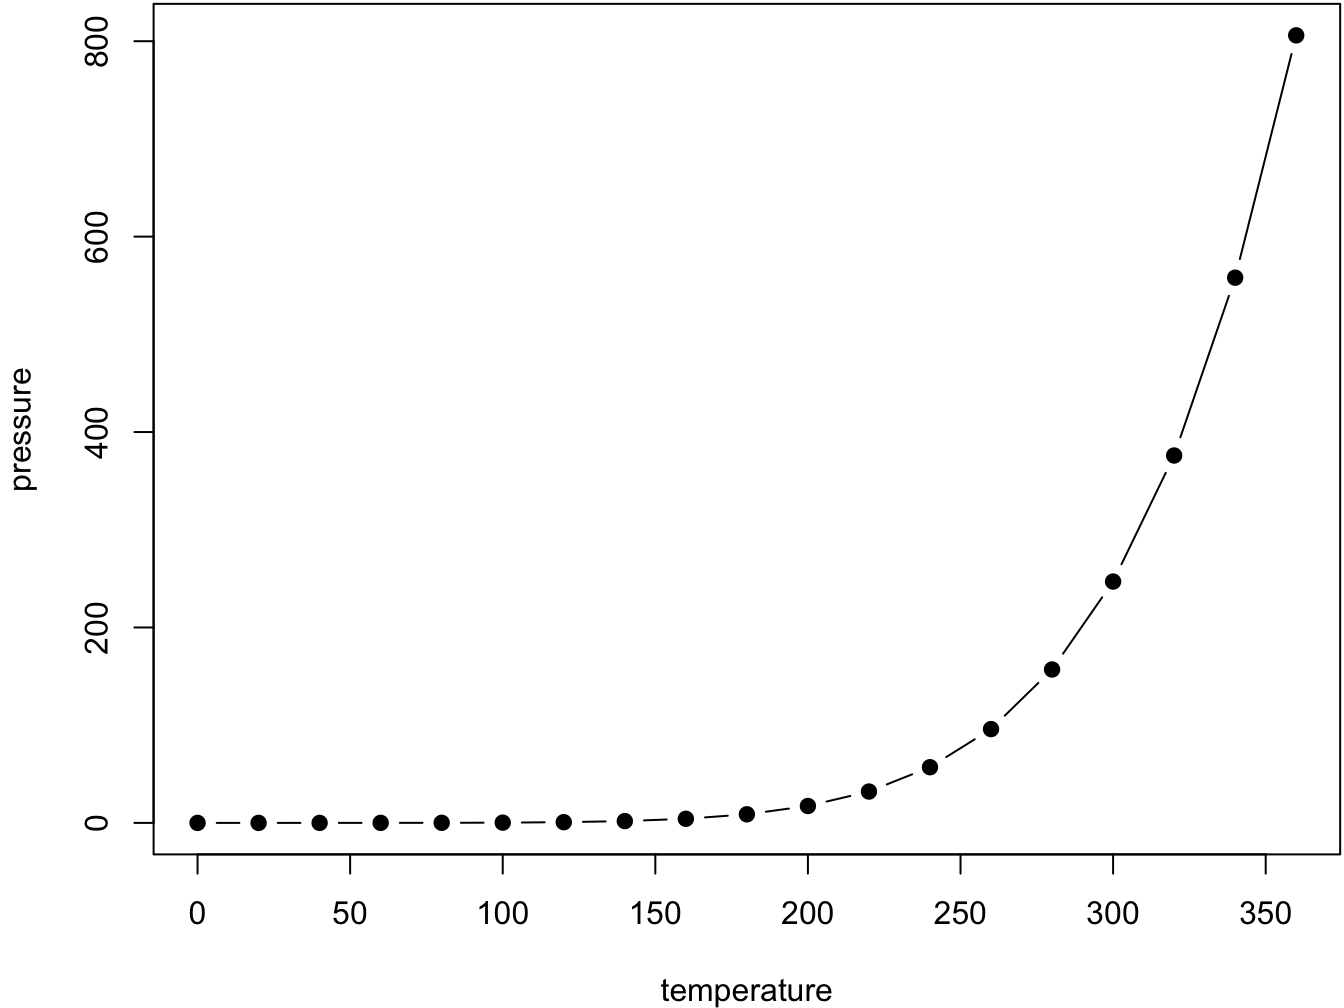
\includegraphics[width=0.8\linewidth]{_main_files/figure-latex/nice-fig-1} 

}

\caption{Here is a nice figure!}\label{fig:nice-fig}
\end{figure}

Don't miss Table \ref{tab:nice-tab}.

\begin{Shaded}
\begin{Highlighting}[]
\NormalTok{knitr}\OperatorTok{::}\KeywordTok{kable}\NormalTok{(}
  \KeywordTok{head}\NormalTok{(pressure, }\DecValTok{10}\NormalTok{), }\DataTypeTok{caption =} \StringTok{'Here is a nice table!'}\NormalTok{,}
  \DataTypeTok{booktabs =} \OtherTok{TRUE}
\NormalTok{)}
\end{Highlighting}
\end{Shaded}

\begin{table}

\caption{\label{tab:nice-tab}Here is a nice table!}
\centering
\begin{tabular}[t]{rr}
\toprule
temperature & pressure\\
\midrule
0 & 0.0002\\
20 & 0.0012\\
40 & 0.0060\\
60 & 0.0300\\
80 & 0.0900\\
\addlinespace
100 & 0.2700\\
120 & 0.7500\\
140 & 1.8500\\
160 & 4.2000\\
180 & 8.8000\\
\bottomrule
\end{tabular}
\end{table}

\hypertarget{parts}{%
\chapter{Parts}\label{parts}}

You can add parts to organize one or more book chapters together. Parts can be inserted at the top of an .Rmd file, before the first-level chapter heading in that same file.

Add a numbered part: \texttt{\#\ (PART)\ Act\ one\ \{-\}} (followed by \texttt{\#\ A\ chapter})

Add an unnumbered part: \texttt{\#\ (PART\textbackslash{}*)\ Act\ one\ \{-\}} (followed by \texttt{\#\ A\ chapter})

Add an appendix as a special kind of un-numbered part: \texttt{\#\ (APPENDIX)\ Other\ stuff\ \{-\}} (followed by \texttt{\#\ A\ chapter}). Chapters in an appendix are prepended with letters instead of numbers.

\hypertarget{footnotes-and-citations}{%
\chapter{Footnotes and citations}\label{footnotes-and-citations}}

\hypertarget{footnotes}{%
\section{Footnotes}\label{footnotes}}

Footnotes are put inside the square brackets after a caret \texttt{\^{}{[}{]}}. Like this one \footnote{This is a footnote.}.

\hypertarget{citations}{%
\section{Citations}\label{citations}}

Reference items in your bibliography file(s) using \texttt{@key}.

For example, we are using the \textbf{bookdown} package \citep{R-bookdown} (check out the last code chunk in index.Rmd to see how this citation key was added) in this sample book, which was built on top of R Markdown and \textbf{knitr} \citep{xie2015} (this citation was added manually in an external file book.bib).
Note that the \texttt{.bib} files need to be listed in the index.Rmd with the YAML \texttt{bibliography} key.

The RStudio Visual Markdown Editor can also make it easier to insert citations: \url{https://rstudio.github.io/visual-markdown-editing/\#/citations}

\hypertarget{blocks}{%
\chapter{Blocks}\label{blocks}}

\hypertarget{equations}{%
\section{Equations}\label{equations}}

Here is an equation.

\begin{equation} 
  f\left(k\right) = \binom{n}{k} p^k\left(1-p\right)^{n-k}
  \label{eq:binom}
\end{equation}

You may refer to using \texttt{\textbackslash{}@ref(eq:binom)}, like see Equation \eqref{eq:binom}.

\hypertarget{theorems-and-proofs}{%
\section{Theorems and proofs}\label{theorems-and-proofs}}

Labeled theorems can be referenced in text using \texttt{\textbackslash{}@ref(thm:tri)}, for example, check out this smart theorem \ref{thm:tri}.

\begin{theorem}
\protect\hypertarget{thm:tri}{}\label{thm:tri}For a right triangle, if \(c\) denotes the \emph{length} of the hypotenuse
and \(a\) and \(b\) denote the lengths of the \textbf{other} two sides, we have
\[a^2 + b^2 = c^2\]
\end{theorem}

Read more here \url{https://bookdown.org/yihui/bookdown/markdown-extensions-by-bookdown.html}.

\hypertarget{callout-blocks}{%
\section{Callout blocks}\label{callout-blocks}}

The R Markdown Cookbook provides more help on how to use custom blocks to design your own callouts: \url{https://bookdown.org/yihui/rmarkdown-cookbook/custom-blocks.html}

\hypertarget{sharing-your-book}{%
\chapter{Sharing your book}\label{sharing-your-book}}

\hypertarget{publishing}{%
\section{Publishing}\label{publishing}}

HTML books can be published online, see: \url{https://bookdown.org/yihui/bookdown/publishing.html}

\hypertarget{pages}{%
\section{404 pages}\label{pages}}

By default, users will be directed to a 404 page if they try to access a webpage that cannot be found. If you'd like to customize your 404 page instead of using the default, you may add either a \texttt{\_404.Rmd} or \texttt{\_404.md} file to your project root and use code and/or Markdown syntax.

\hypertarget{metadata-for-sharing}{%
\section{Metadata for sharing}\label{metadata-for-sharing}}

Bookdown HTML books will provide HTML metadata for social sharing on platforms like Twitter, Facebook, and LinkedIn, using information you provide in the \texttt{index.Rmd} YAML. To setup, set the \texttt{url} for your book and the path to your \texttt{cover-image} file. Your book's \texttt{title} and \texttt{description} are also used.

This \texttt{gitbook} uses the same social sharing data across all chapters in your book- all links shared will look the same.

Specify your book's source repository on GitHub using the \texttt{edit} key under the configuration options in the \texttt{\_output.yml} file, which allows users to suggest an edit by linking to a chapter's source file.

Read more about the features of this output format here:

\url{https://pkgs.rstudio.com/bookdown/reference/gitbook.html}

Or use:

\begin{Shaded}
\begin{Highlighting}[]
\NormalTok{?bookdown}\OperatorTok{::}\NormalTok{gitbook}
\end{Highlighting}
\end{Shaded}

  \bibliography{book.bib,packages.bib}

\end{document}
